\documentclass[12pt, openany]{book}
%\documentclass[12pt,oneside]{book}
\usepackage{lipsum}
\usepackage[a4paper,top=2cm,bottom=2cm,inner=3cm,outer=1cm,marginparwidth=4cm]{geometry}
\usepackage{titlesec}
\usepackage{titling}
\usepackage{fontspec}
\usepackage{suffix}
\usepackage{multicol}
\usepackage{tikz}
\usepackage{pdflscape}
\usepackage{onimage} % loaded to print tikz on images
\usepackage{bm}
\usepackage{textcomp}
\usepackage{gensymb}
\usepackage{enumitem}

% ---- watermark
\usepackage{eso-pic}
\newcommand\FrontPic{%
\put(0,0){%
\parbox[b][\paperheight]{\paperwidth}{%
\vspace*{.3\paperheight}
\flushleft
\includegraphics[height=.7\paperheight,%
keepaspectratio]{img/front.png}%
\vfill
}}}

\newcommand\BackPic{%
\put(0,0){%
\parbox[b][\paperheight]{\paperwidth}{%
\vspace*{.3\paperheight}
\flushright
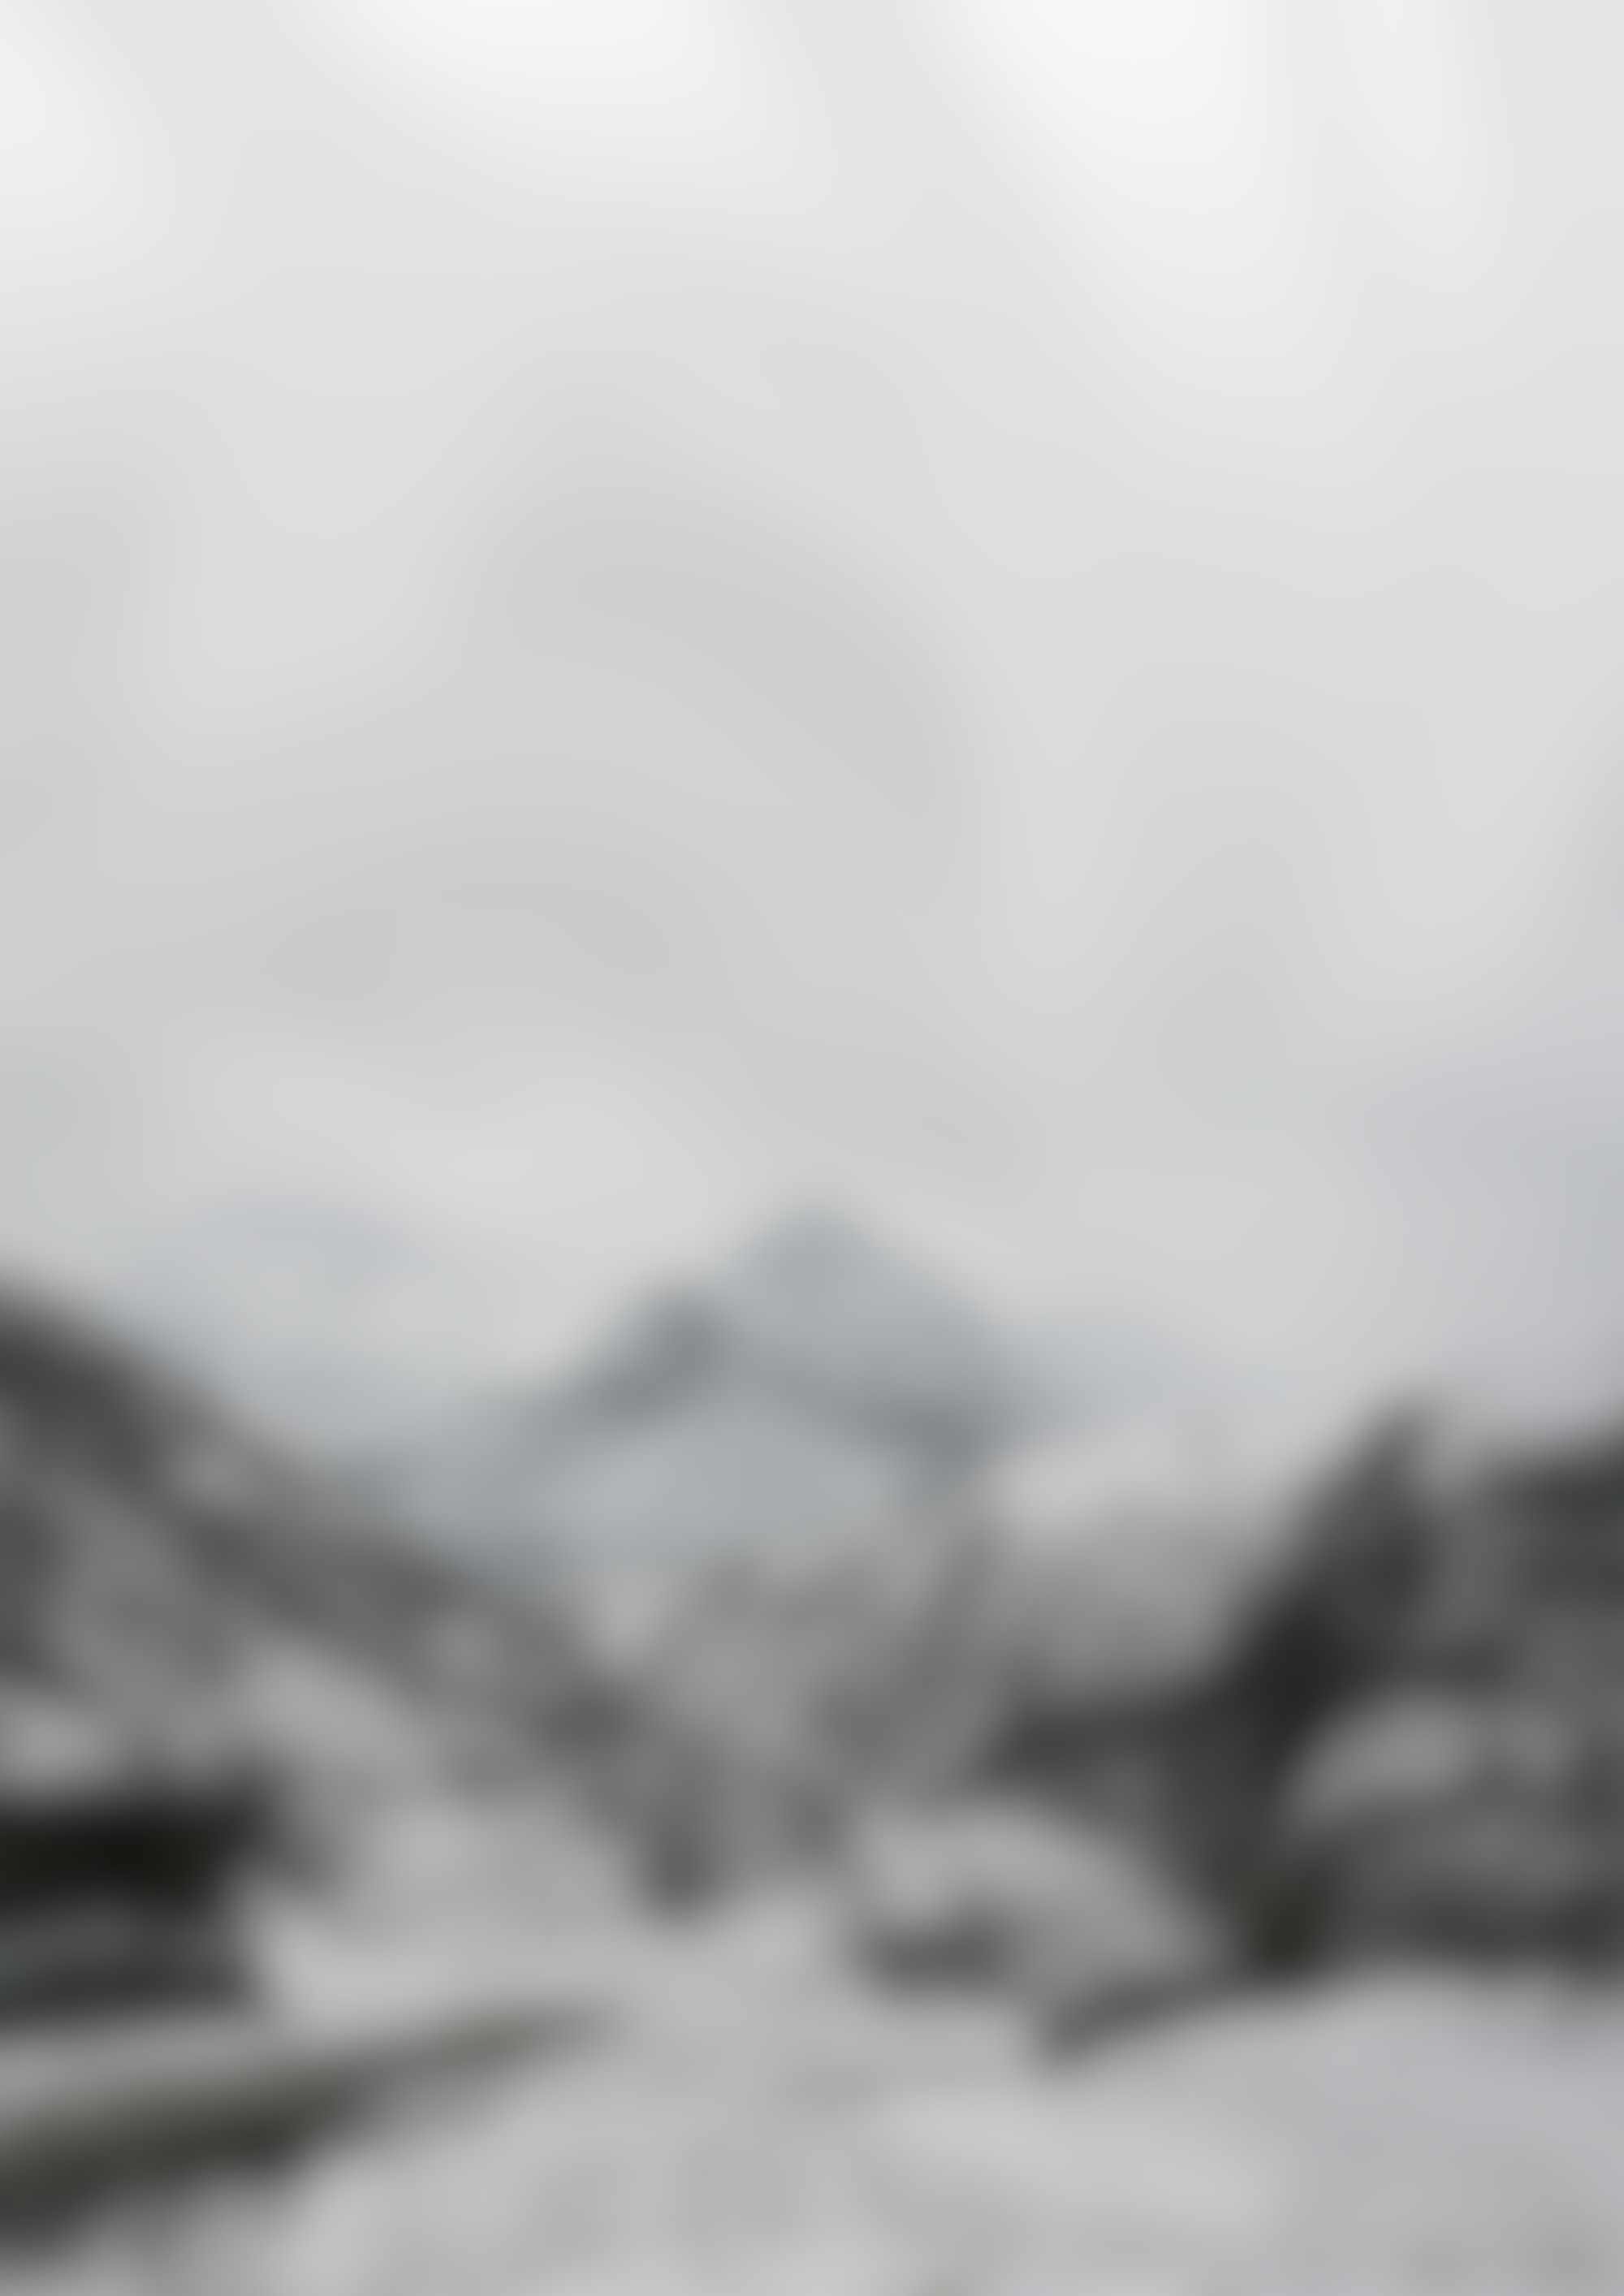
\includegraphics[height=.7\paperheight,%
keepaspectratio]{img/back.png}%
\vfill
}}}

\newcommand{\NewPic}[1]{
\put(0,0){%
\parbox[b][\paperheight]{\paperwidth}{%
\vspace*{.22\paperheight}
\flushright
\includegraphics[width=1\paperwidth,%
keepaspectratio]{#1}%
\vfill
}}}

\newcommand{\NewPicHeight}[2]{
\put(0,0){%
\parbox[b][\paperheight]{\paperwidth}{%
\vspace*{#2}
\flushright
\includegraphics[width=1\paperwidth,%
keepaspectratio]{#1}%
\vfill
}}}

\usepackage{xcolor}%,sectsty}
\definecolor{clrt1}{RGB}{215, 95, 95}    % color 1
\definecolor{clrt2}{RGB}{135, 175, 135}  % color 2
%\definecolor{clrt1}{RGB}{80, 80, 80}    % gray 1
%\definecolor{clrt2}{RGB}{180, 180, 180}  % gray 2

\usepackage{tocloft}
\renewcommand{\cftchapfont}{\color{clrt1}}
\renewcommand{\cftsecfont}{\color{clrt2}}

\newcommand\chapterauthor[5]{\authortoc{#1}{#4}{#5}\noindent\printchapterauthor{#1}{#2}{#3}}
\WithSuffix\newcommand\chapterauthor*[1]{\printchapterauthor{#1}{}{}}

\makeatletter
\newcommand{\printchapterauthor}[3]{%
  {%\vspace*{-25pt}%
  %\linespread{1.5}
  \large#1$^{~\small\textnormal#2}$#3%
  %\par\nobreak\vspace*{30pt}
  }
  \@afterheading%
}

\newcommand{\authortoc}[3]{%
  \addtocontents{toc}{\hspace{#2em}}%\vskip-10pt}%
  \addtocontents{toc}{
    {\protect\scriptsize\textcolor{black}{#1#3}}{}{}
    }
  %\addtocontents{toc}{\vskip5pt}%
}

\setmainfont{Charter}[
  Path=./fnt-charter/,
  Extension=.ttf,
  UprightFont=*-Regular,
  BoldFont=*-Bold,
  ItalicFont=*-Italic,
  BoldItalicFont=*-Bold-Italic
]

\usepackage{titling}

% paragraph formating -----------
\setlength\fboxsep{.6em}
\setlength{\parskip}{.8em} % vertical spcae
\setlength{\parindent}{0em} % vertical spcae
\renewcommand{\baselinestretch}{1.2} 

\newcommand{\headchapter}{}

\usepackage{fancyhdr}
 \setlength{\headheight}{15pt} 
\pagestyle{fancy}
\fancyhf{}
%\rhead{\chaptername \headchapter}
\fancyhead[RO, LE] {\chaptername \headchapter}
\cfoot{--~\thepage~--}

\newcommand\mystyleone{%
\fancyhf{}
%\rhead{\chaptername \headchapter}
\fancyhead[RO, LE] {\chaptername \headchapter}
\cfoot{--~\thepage~--}
}
 
\newcommand\mystyletwo{%
   \cfoot{--~\thepage~--}
}


%title formatin (margins)
\titlespacing\chapter{0pt}{0em plus 4pt minus 2pt}{1em plus 2pt minus 2pt}
\titleformat{\chapter}{\Huge\normalfont\bfseries\color{clrt1}}{}{0em}{\hfil{--\hspace*{.25em}\thechapter\hspace*{.25em}-- }\\}
\titleformat{\section}{\large\bfseries\color{clrt2}}{\thesection.}{0.5em}{}
% table formats  -----------
\usepackage{multirow}
\usepackage{multicol}
\usepackage{colortbl}
\usepackage{array}
\newcolumntype{L}[1]{>{\raggedright\let\newline\\\arraybackslash\hspace{0pt}}m{#1}}
\newcolumntype{C}[1]{>{\centering\let\newline\\\arraybackslash\hspace{0pt}}m{#1}}
\newcolumntype{R}[1]{>{\raggedleft\let\newline\\\arraybackslash\hspace{0pt}}m{#1}}

% citation management -----------
\newcommand{\cc}[1]{\textcolor{clrt2!80}{#1}}
\newcommand{\gitref}{\hyperlink{git}{git}}
\newcommand{\textsw}[1]{\textcolor{darkgray}{\textsc{#1}}}
\newcommand{\overbar}[1]{\mkern 1.5mu\overline{\mkern-1.5mu#1\mkern-1.5mu}\mkern 1.5mu}
\newcommand*\mean[1]{\overbar{#1}}

\usepackage{hyperref}
\hypersetup{
    colorlinks,
    linkcolor={black!60},
    citecolor={black!60},
    urlcolor={black!60}}

% bibliography management -----------
% inline citations
\usepackage{csquotes}
\makeatletter
%Take the original environment definition and change the leftmargin to 1cm
\renewenvironment*{displayquote}
  {\begingroup\setlength{\leftmargini}{1.3em}\csq@getcargs{\csq@bdquote{}{}}}
  {\csq@edquote\endgroup}
\makeatother

\usepackage{bibentry}
\usepackage{natbib}  %set citing format
\bibliographystyle{apalike}
%\makeatletter 
%\renewcommand\@biblabel[1]{#1.} 
%\makeatother
\usepackage{multibib}
\newcites{at}{\normalsize\textcolor{black}{Original publication}}
\newcites{am}{Chapter 1 References}

\newcites{bt}{\normalsize\textcolor{black}{Original publication}}
\newcites{bm}{Chapter 2 References}

\newcites{ct}{\normalsize\textcolor{black}{Original publication}}
\newcites{cm}{Chapter 3 References}

\newcites{dt}{\normalsize\textcolor{black}{Original publication}}
\newcites{dm}{Chapter 4 References}

\newcites{im}{Intro References}
\newcites{zm}{Synthesis References}

\usepackage{etoolbox}
\makeatletter
\providecommand{\bibname}{Bibliography}
\providecommand{\refname}{References}
\@ifpackageloaded{natbib}
  {\renewcommand{\bibsection}{%
    \@ifundefined{chapter}
    {\subsection*{\refname \markboth{\refname}{\bibname}%
    \addcontentsline{toc}{subsection}{\refname}}
    }
    {\section*{\refname \markboth{\refname}{\bibname}%
    \addcontentsline{toc}{section}{\refname}}
    }
  }}
  {\@ifundefined{chapter}
    {\patchcmd{\thebibliography}{\section*{\refname}}{%
      \subsection*{\refname}
      \addcontentsline{toc}{subsection}{\refname}
      }{}{}
    }
    {\patchcmd{\thebibliography}{\chapter*{\bibname}}{%
      \section*{\refname}
      \addcontentsline{toc}{section}{\refname}
      }{}{}
    }
  }
\@ifundefined{chapter}
  {\newcommand{\bibliographies}{%
  \section*{\bibname}
  \if@FMB@addtotoc\addcontentsline{toc}{section}{\bibname}\fi}}
  {\newcommand{\bibliographies}{%
  \chapter*{\bibname}
  \if@FMB@addtotoc\addcontentsline{toc}{chapter}{\bibname}\fi}}
\makeatother

% figure/table management -----------
\usepackage{floatrow}
\usepackage[figurename=Figure,tablename=Table,labelfont=bf,format=plain, font=footnotesize]{caption} 
\captionsetup[figure]{labelfont={bf},labelformat={default},labelsep=colon}
\floatsetup[table]{capposition=top}

\newcounter{figS}
\newcommand{\figS}[1]{\refstepcounter{figS}\label{#1}}
\newcounter{tabS}
\newcommand{\tabS}[1]{\refstepcounter{tabS}\label{#1}}

\newcommand{\figref}[1]{\hyperref[#1]{Figure~\ref{#1}}}
\newcommand{\tabref}[1]{\hyperref[#1]{Table~\ref{#1}}}
\newcommand{\figrefS}[1]{\hyperref[#1]{Suppl. Fig.~\ref{#1}}}
\newcommand{\tabrefS}[1]{\hyperref[#1]{Suppl. Tab.~\ref{#1}}}

\usepackage{placeins}
\DeclareFloatingEnvironment[
  fileext=losf,
  listname={List of Supplementary Figures},
  name=Suppl.~Figure
]{supplFigure}

\DeclareFloatingEnvironment[
  fileext=lost,
  listname={List of Supplementary Tables},
  name=Suppl.~Table
]{supplTable}


\newlength{\fwidth}
\setlength{\fwidth}{168.36mm}%{183mm}
\newlength{\fheight}
\setlength{\fheight}{261.28mm}%{284mm}

\titlespacing*{\chapter}{0pt}{-50pt}{40pt}

\usepackage{morewrites}
%take out later
\usepackage{colortbl}
\definecolor{annoGRAY}{RGB}{240,240,240}
\definecolor{annoDGRAY}{RGB}{200,200,200}
\newcommand{\gene}[1]{\textit{\MakeLowercase{#1}}}

%\renewcommand{\cftloftitlefont} {\MakeUppercase{\large\bfseries}}
%\renewcommand{\cftlottitlefont} {\MakeUppercase{\large\bfseries}}
\renewcommand{\listfigurename}{\textcolor{clrt2}{\large\textbf{List of Figures}}}
\renewcommand{\listsupplFigurename}{\textcolor{clrt2}{\large\textbf{List of Supplementary Figures}}}

\renewcommand{\listtablename}{\textcolor{clrt2}{\large\textbf{List of Tables}}}
\renewcommand{\listsupplTablename}{\textcolor{clrt2}{\large\textbf{List of Supplementary Tables}}}

% keep last line of paragraph justified
\newcommand{\startsquarepar}{%
    \par\begingroup \parfillskip 0pt \relax}
\newcommand{\stopsquarepar}{%
    \par\endgroup}
    
\usepackage[most]{tcolorbox}

\newcommand{\projanticase}[1]{\MakeUppercase{#1}}
\newcommand{\projcase}[1]{\MakeLowercase{#1}}
\usepackage{amssymb}

\newcommand\blankpage{%
    \clearpage\thispagestyle{empty}\mbox{}\clearpage
%    \addtocounter{page}{-1}%
    \newpage}

\def\MYTITLE{The Thesis Title}
\def\MYAUTHOR{Author Name}
\title{\MYTITLE}

\begin{document}
\thispagestyle{empty}
\AddToShipoutPicture*{\PagePic{images/title.jpg}}
%\AddToShipoutPicture*{\FrontPic}
\newgeometry{top=2.5cm, bottom=2cm, inner=2.25cm, outer=1.75cm}
%\newgeometry{top=2.5cm, bottom=2cm, inner=2cm, outer=2cm}
\begin{center}
\begin{LARGE}
\vspace*{1.2em}
{\huge\textbf{\textcolor{clrt1}{\thetitle}}}\\
\vspace*{.1\paperheight}
\MYAUTHOR
\end{LARGE}
\end{center}
\vfill

\blankpage

\newpage
\thispagestyle{empty}

\newgeometry{top=2.5cm, bottom=2cm, inner=2.25cm, outer=1.75cm}

\begin{center}
\begin{LARGE}
\vspace*{1.2em}
\textbf{\thetitle}\\
\end{LARGE}
\vfill
Dissertation
zur Erlangung des akademischen Grades\\\vspace*{2em}
\textit{Doctor rerum naturalium}\\\vspace*{2em}
der Mathematisch-Naturwissenschaftlichen Fakultät\\
der Christian-Albrechts-Universität zu Kiel\\\vspace*{2em}
vorgelegt von\\
\MYAUTHOR\\\vspace*{2em}
Kiel, XX.XX.20XX
\end{center}

\blankpage
\thispagestyle{empty}
~\vfill

\hfill\begin{tabular}{rl}
    Erster Gutachter: & Prof. XX \\
    Zweite Gutachterin: & Prof. XX \\
    Tag der Disputation: & XX.XX.20XX\\
    Zum Druck genehmigt: & XX.XX.20XX
\end{tabular}{}

\blankpage
\newpage
\renewcommand{\chaptername}{}
\setcounter{page}{1}
\tableofcontents

\newpage
\renewcommand{\chaptername}{}
\renewcommand{\headchapter}{Summary}
\section*{Summary}
\addcontentsline{toc}{section}{Summary}

Here lives the summary of the thesis ($\sim$ 1 -- 2 pages)

\textcolor{black!35}{\lipsum[1]}

\newpage

\section*{Zusammenfassung}
\addcontentsline{toc}{section}{Zusammenfassung}

Here lives the German version of the summary (also $\sim$ 1 -- 2 pages)

\textcolor{black!35}{\lipsum[1]}


\setcounter{chapter}{-1}
\chapter[Introduction]{\centering Introduction\\}
\renewcommand{\headchapter}{Introduction}
% add your introduction section here ...
``\textit{This includes examples of quotes, the inclusion and reference to a Figure, a (chapter-specific) citation and a summary box.}''\\
\hspace*{.83\textwidth}{\citepim{Darwin1859}} %note the section-specific citation commands (indication section and within text (i/a/b/c/z), and self reference from the chapter title (p/m))

\begin{multicols}{2}
\begin{figure*}[!hb] % figure will be placed after the next paragraph finishes
\centering
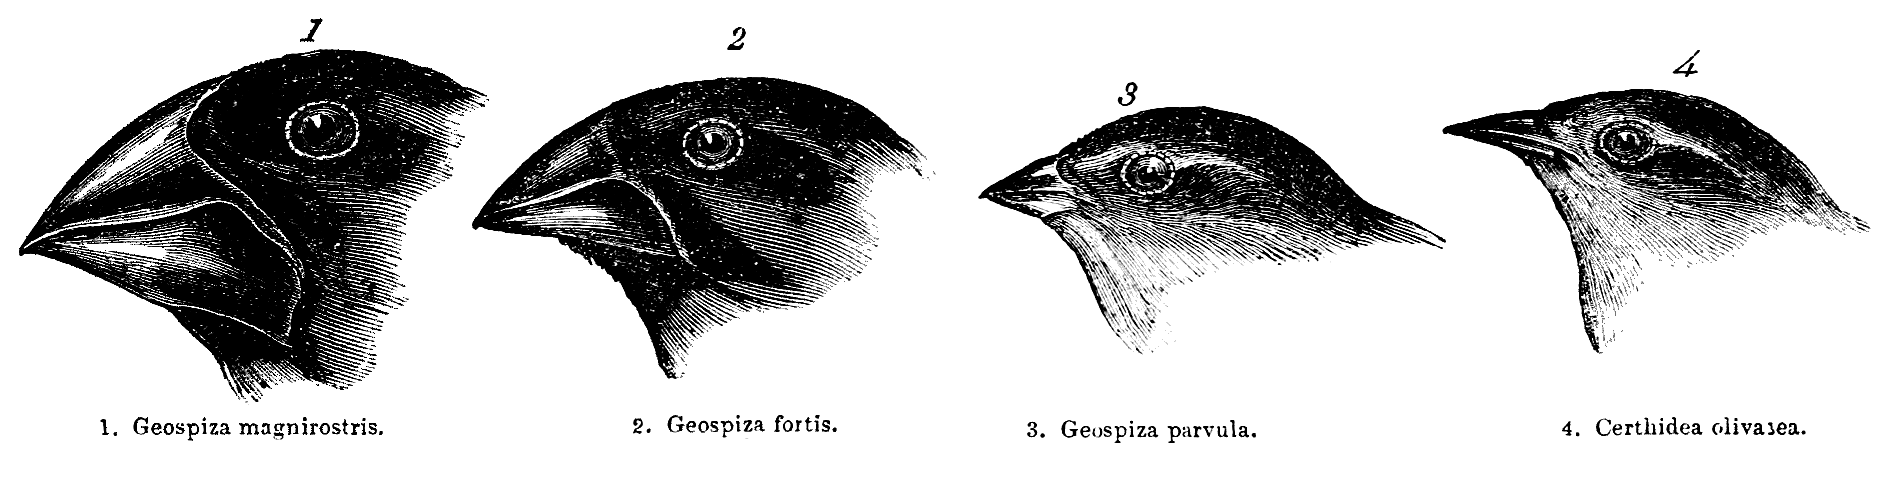
\includegraphics[width = \fwidth]{figures/ci/finches.png}
\caption[Darwins Finches]{\label{fig:cif1}\textbf{Darwins Finches.} These are such famous birds.
}
\end{figure*}

\section{First Section}

\textbf{Inline Quotes:} By the way, we can also quote \textit{in line} using the environment \texttt{$\backslash$displayquote}:

\begin{displayquote}
\textit{
I look at the term species, as one arbitrarily given for the sake of convenience to a set of individuals closely resembling each other [...].}
\hfill{\citepim{Darwin1859}}
\end{displayquote}

\textbf{Adding Figures:}
Figures are added to the text using the \texttt{figure*} environment in combination with the \texttt{$\backslash$includegraphics} command (s. example in source code).
You can also use the \texttt{$\backslash$label} command to add a tag to the figure which you can use to refernce the figure in your text.
Note that figures will show up somewhere \textit{after} the paragraph that follows the \textsw{figure*} environment. If you need to force the appearance on a specific page you can use the command \texttt{$\backslash$FloatBarrier}.

Here is some demonstration how to reference a Figure (using the label from the figure command) --- just look at these birds (\figref{fig:cif1}).
The reference is done using the command \texttt{$\backslash$figref\{\}}.

\textbf{Landscape Figures:} For figures in \textit{landscape mode}, use the \texttt{landscape} environment.
I usually do this in the following manner:

\begin{tcolorbox}[arc=0pt,outer arc=0pt,breakable,colback=black!05,colframe=black!10,pad at break=2mm,boxrule=0.1pt]
\begin{lstlisting}
\begin{|\cc{landscape}|}
\begin{|\dd{figure}|}[!ht]
 \centering
 \includegraphics{path/figure}
 \caption[LOF-title]{
  \label{fig:lab}
  \textbf{Caption Title.}
  Caption ...
  }
\end{|\dd{figure}|}
\end{|\cc{landscape}|}
\end{lstlisting}
\end{tcolorbox}

Also, note the difference between normal mode (\texttt{figure*}) and landscape mode (\texttt{figure}):
All \texttt{Float}-environments (\texttt{figure}, \texttt{supplFigure}, \texttt{table} and \texttt{supplTable}) that you want to place within a \texttt{multicols} text, need to have an  appended asterisk.

To embed a landscape figure within the text, the overall approach is:

\begin{tcolorbox}[arc=0pt,outer arc=0pt,breakable,colback=black!05,colframe=black!10,pad at break=2mm,boxrule=0.1pt]
\begin{lstlisting}
|\textnormal{\textcolor{black!35}{this long sentence of running text is not}}|
\stopsquarepar
\end{|\dd{multicols}|}

\begin{|\cc{landscape}|}
 ...
\end{|\cc{landscape}|}
\begin{|\dd{multicols}|}{2}
|\textnormal{\textcolor{black!35}{finished yet, but wraps around ...}}|
\end{lstlisting}
\end{tcolorbox}

Unfortunately, breaking the text around landscape figures needs to be done manually --- finding the best break is usually done last because any change in the text afterwards might result in awkward half-empty pages.
Also, note the \texttt{$\backslash$stopsquarepar}, which is used to cause the text-justification to behave as if the the text was not broken (keeping eg. the block-justification intact).

\section{Second Section}

The rest is just dummy text....

\lipsum[1]

\begin{tcolorbox}[arc=0pt,outer arc=0pt,breakable,title = Summary,
colback=clrt2!30,colframe=clrt2,pad at break=3mm,boxrule=1pt]
   \begin{itemize}[leftmargin=1em]
   %\setlength{\itemindent}{-1em}
   \setlength{\itemsep}{0em}
    \item{Quotes can either come as \textit{opening} or \textit{inline} quotes.}
    \item{The reference to figures happens via the command \textsw{$\backslash figref\{\}$}.}
    \item{Summary boxes can be added using the \textsw{tcolorbox} environment.}
\end{itemize}
\end{tcolorbox}

\bibliographystyleim{apalikeK}
\bibliographyim{library/ci.bib}
\end{multicols}


\newpage
\renewcommand{\chaptername}{Chapter~}
\renewcommand{\headchapter}{\thechapter}
% here live the intros to all the individual chapters
% also, you can toggle the inclusion of the individual 
% chapters (by commenting the \input{ch_c1.txt}) for a 
% faster build of the document during preparation

% use the brackets [] to use different formating in the text vs. the TOC 
\chapter[This is the very very, oh sooo very long title of Chapter 1 --- it even needs line breaks]{\centering This is the very very, oh sooo very long\\ title of Chapter1 --- it even needs line breaks}
\vfill

\chapterauthor{\textbf{First Author}}{1}{,}{1.3}{,}
\chapterauthor{Second Author}{2}{,}{0}{,}
\chapterauthor{Third Author}{3}{, \smallskip}{0}{,}
\chapterauthor{Fourth Author}{1}{\vspace*{-.5em}\\}{0}{}

\noindent\begin{tabular}{L{.015\textwidth}L{.985\textwidth}}
    1 & First Research Institute \\
    2 & Second Research Institute \\
    3 & Third Research Institute
\end{tabular}

\noindent\colorbox{clrt1!15}{\parbox{\textwidth}{
This study was originally published in \textit{Name of the Journal}.
Figures were re-drawn for this thesis but no additional changes were made.
The re-print within this thesis is in agreement with \textit{Name of the Publisher} under license number \textit{XX}.

\nociteat{ref1}
\bibliographystyleat{apalikeK}
\bibliographyat{library/chapters.bib}
}}

\noindent\section*{Abstract}
This includes a demo of a Supplementary Figure, the \textit{narrow mode} which works for Figures and Supplementary Figure and use a chapter-specific citation.

\noindent{\bf Keywords:} Key1, Key2, Key3.

\begin{multicols}{2}
\section{Introduction}
\noindent
Here again, we showcase some old stuff that needs a (chapter-specific) citation \citepam{Darwin1859}.
Also, note the slight variation in referencing Supplementary Figures (\figrefS{fig:c1s1}) using \textsw{$\backslash figrefS\{\}$} (vs. \textsw{$\backslash figref\{\}$}).
Then again, it is time for dummy text: 

\section{A section}
% demo of a supplementary figure (in "narrow mode" )
\begin{supplFigure*}[!t]
\floatbox[{\capbeside\thisfloatsetup{capbesideposition={left,center},capbesidewidth=.5\fwidth}}]{supplFigure}[\FBwidth]
{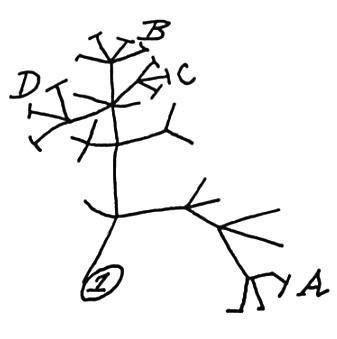
\includegraphics[width = .5\fwidth]{figures/c1/tree.jpg}}
{\caption[Darwins tree]{\label{fig:c1s1}\textbf{Darwins tree.}
Oh, the fame...}}
\end{supplFigure*}


\lipsum[2-6] 

\bibliographystyleam{apalike}
\bibliographyam{library/c1.bib}
\end{multicols}

\chapter[Short title of Chapter 2]{\centering Short title of Chapter 2\\}

\chapterauthor{\textbf{First Author}}{1}{,}{1.3}{,}
\chapterauthor{Second Author}{2}{,}{0}{,}
\chapterauthor{Third Author}{3}{, \smallskip}{0}{,}

\noindent\begin{tabular}{L{.015\textwidth}L{.985\textwidth}}
    1 & First Research Institute \\
    2 & Second Research Institute \\
    3 & Third Research Institute
\end{tabular}

\noindent\colorbox{clrt1!15}{\parbox{\textwidth}{
This study was originally published in \textit{Name of the Journal}.
Figures were re-drawn for this thesis but no additional changes were made.
The re-print within this thesis is in agreement with \textit{Name of the Publisher} as the original publication is under Creative Commons CC BY license.

\nocitebt{ref2}
\bibliographystylebt{apalikeK}
\bibliographybt{library/chapters.bib}
}}

\section*{Abstract}
\noindent
Here, we talk about different citation styles and look at tabels.

\noindent{\bf Keywords:} Key1, key2, key3.

\begin{multicols}{2}

\begin{table*}[!htb]
\centering
\caption[Summary of Anderson's Iris Data]{\label{tab:c2t1}
A small summary of Edgar Anderson's Iris Data as implemented in R.}
\begin{small}
\arrayrulecolor{black!25}
\begin{tabular}{ r | c c | c c }
\arrayrulecolor{black}
\hline
\arrayrulecolor{black!25}
\multirow{2}{*}{\textbf{Species}} &\multicolumn{2}{c|}{\textbf{Sepal}}&\multicolumn{2}{c}{\textbf{Petal}}\\
& \textbf{Avg. Length} & \textbf{Avg. Width} & \textbf{Avg. Length} & \textbf{Avg. Width}\\
\arrayrulecolor{black}\hline
\textit{I. setosa}&5.01&3.428&1.46&0.246\\
\textit{I. versicolor}&5.94&2.77&4.26&1.33\\
\textit{I. irginica}&6.59&2.974&5.55&2.03\\\hline\hline
\end{tabular}

\end{small}
\end{table*}

\section{Introduction}

So, as far as citations go, I use a modular command system: This is based on the basic \LaTeX - citation commands (\textsw{$\backslash cite$}, \textsw{$\backslash citep$} and \textsw{$\backslash citealt$}) and two single-letter suffixes (i/a/b/c/d/z and t/m). The first letter indicates the current section (Intro: I, Chapter 1:a, 2:b, Synthesis:z), while the last letter indicates whether this is the self-citation from the Chapter title page (t) or a citation within the manuscript (m).
Form these pieces, the actual commands can be puzzled together, with the actual commands looking something like \textsw{$\backslash citepcm\{\}$}.

So, you might remember that in the first Chapter \citepbm{ref1}, we cited \citebm{Darwin1859} a lot.
Now in this chapter we are going to look at the data from \citealtbm{Anderson35}.
We are going to show a summary of this data in a main table (\tabref{tab:c2t1}), while a glimpse of the actual data structure is given in a Supplemental Table (\tabrefS{tab:c2st1}).
The referencing of the tables happens using the commands \textsw{$\backslash tabref\{\}$} and \textsw{$\backslash tabrefS\{\}$}.

\section{First Section}
\lipsum[7-9]

\begin{supplTable*}[!t]
\centering
\captionsetup{width=.6\linewidth}
\caption[Subset of Anderson's Iris Data]{\label{tab:c2st1}
A subset of Edgar Anderson's Iris Data as implemented in R.}
\begin{small}
\begin{tabular}{ r c c c c }
Species&Sepal Length&Sepal Width&Petal Length&Petal Width\\\hline
\textit{I. setosa}&5.4&3.4&1.7&0.2\\
\textit{I. setosa}&5.4&3.7&1.5&0.2\\
\textit{I. setosa}&5.7&3.8&1.7&0.3\\
\textit{I. setosa}&5.1&3.5&1.4&0.2\\
\textit{I. setosa}&4.8&3&1.4&0.3\\
\textit{I. setosa}&5.1&3.3&1.7&0.5\\\arrayrulecolor{black!25}\hline
\textit{I. versicolor}&5.8&2.6&4.0&1.2\\
\textit{I. versicolor}&5.8&2.7&3.9&1.2\\
\textit{I. versicolor}&5.5&2.3&4.0&1.3\\
\textit{I. versicolor}&6.0&2.7&5.1&1.6\\
\textit{I. versicolor}&5.6&3.0&4.5&1.5\\
\textit{I. versicolor}&6.3&3.3&4.7&1.6\\\hline
\textit{I. virginica}&6.9&3.2&5.7&2.3\\
\textit{I. virginica}&7.2&3.2&6.0&1.8\\
\textit{I. virginica}&6.5&3.0&5.5&1.8\\
\textit{I. virginica}&5.8&2.7&5.1&1.9\\
\textit{I. virginica}&6.3&3.4&5.6&2.4\\
\textit{I. virginica}&7.7&2.6&6.9&2.3\\\arrayrulecolor{black}\hline
\end{tabular}

\end{small}
\end{supplTable*}

\section{Second Section}
\lipsum[10-12]

\section*{Acknowledgments}

We thank all the nice people.

\bibliographystylebm{apalike}
\bibliographybm{library/c2.bib}
\end{multicols}



\chapter[Synthesis]{\centering Synthesis\\}
\renewcommand{\chaptername}{}
\renewcommand{\headchapter}{Synthesis}
\begin{multicols}{2}
\section{Synthesis}

\subsection*{Final Section}

We always need to cite \citealtzm{Darwin1859}.

\textcolor{black!35}{\lipsum[1-3]}

\bibliographystylezm{apalikeK}
\bibliographyzm{library/cz.bib}
\end{multicols}

\newpage
%\thispagestyle{fancy}
\renewcommand{\chaptername}{}
\mystyletwo
\renewcommand{\headchapter}{Lists}
{\Huge\normalfont\bfseries\textcolor{clrt1}{Appendix}}
\addcontentsline{toc}{chapter}{Appendix}
\addcontentsline{toc}{section}{List of Figures}
\listoffigures
\addcontentsline{toc}{section}{List of Supplementary Figures}
\listofsupplFigures
\addcontentsline{toc}{section}{List of Tables}
\listoftables
\addcontentsline{toc}{section}{List of Supplementary Tables}
\listofsupplTables

\newpage
\mystyleone
\renewcommand{\headchapter}{Author Contributions}
\section*{Declaration of Author Contributions}
\addcontentsline{toc}{section}{Declaration of Author Contributions}

\textbf{Chapter~1:}\\

\textbf{Chapter~2:}\\


\newpage
\renewcommand{\headchapter}{CV}
\section*{Curriculum Vitae}
\addcontentsline{toc}{section}{Curriculum Vitae}

%{\HorRule\vspace*{2mm}}
\begin{tabular}{@{}p{.18\textwidth}p{.32\textwidth}p{.15\textwidth}p{.35\textwidth}p{.15\textwidth}p{.35\textwidth}p{.15\textwidth}p{.35\textwidth}}
\noalign{\smallskip}
		\textbf{Name:} 	& \MYAUTHOR \hspace{3.5cm} & \textbf{Nationality:} & XX \\ 
		\textbf{Birthday:}	& XX.XX.19XX &  \textbf{Orcid-id}&\href{https://orcid.org/XX}{XX}\\
		\textbf{Place of birth:} & XX&&\\\
\end{tabular}

\vspace*{-1em}
\subsection*{Education in Science}
\begin{tabular}{@{}rl}
			\textbf{since 20XX/XX/XX} & Doctoral candidate at the \textit{XX Lab} \\
			& XX Institute\\
			\noalign{\smallskip}
			\textbf{20XX/XX/XX - 20XX/XX/XX} & Master student (M.Sc. XX) \\
			& XX University\\
			\noalign{\smallskip}
			\textbf{20XX/XX/XX - 20XX/XX/XX} & Bachelor student (B.Sc. XX)\\
					& XX University\\
\end{tabular}

\subsection*{Practical Experience in Science/ Teaching}
\begin{tabular}{@{}p{.2\textwidth}p{.8\textwidth}}
            \textbf{20XX/ XX-XX} & Teaching assistant at XX\\
			& Location, County. \textit{XX University}\\
			\noalign{\smallskip}
            \textbf{20XX/ XX-XX} & Field Trip\\
			& Location, County. \textit{XX University}\\
\end{tabular}


\newpage
\renewcommand{\headchapter}{Acknowledgments}
\section*{Acknowledgments}
\addcontentsline{toc}{section}{Acknowledgments}
% put the acknowledgments here ...
I would like to thank ...

%\blankpage
\newpage
\renewcommand{\headchapter}{~}
\section*{Eidesstattliche Erklärung}
\addcontentsline{toc}{section}{Eidesstattliche Erklärung}
Hiermit bestätige ich, \MYAUTHOR, dass die folgende Dissertation\vspace{1em}

\textit{\MYTITLE}\vspace{1em}

von mir, unter Beratung meines Betreuers, selbstständig verfasst wurde, nach Inhalt und Form meine eigene Arbeit ist und keine weiteren Quellen und Hilfsmittel als die angegebenen verwendet wurden.

\noindent{}Die vorliegende Arbeit ist unter Einhaltung der Regeln guter wissenschaftlicher Praxis der Deutschen Forschungsgemeinschaft entstanden und wurde nicht im Rahmen eines Prüfungsverfahrens an anderer Stelle vorgelegt.
Veröffentlichte oder zur Veröffentlichung eingereichte Manuskripte wurden kenntlich gemacht.
Mir wurde kein akadamischer Grad entzogen\\\vspace{.07\paperheight}

\noindent{}XX, XX.XX.20XX\hfill{}\rule{.25\textwidth}{0.4pt}

\hfill{}\MYAUTHOR\hspace*{.04\textwidth}\\

%\blankpage
\newpage
\AddToShipoutPicture*{\PagePic{images/back.jpg}}
\thispagestyle{empty}
\textcolor{white!90}{\hrule}\vspace*{1em}
\vfill

\textcolor{white!90}{\hrule}\vspace*{.15em}
\hfil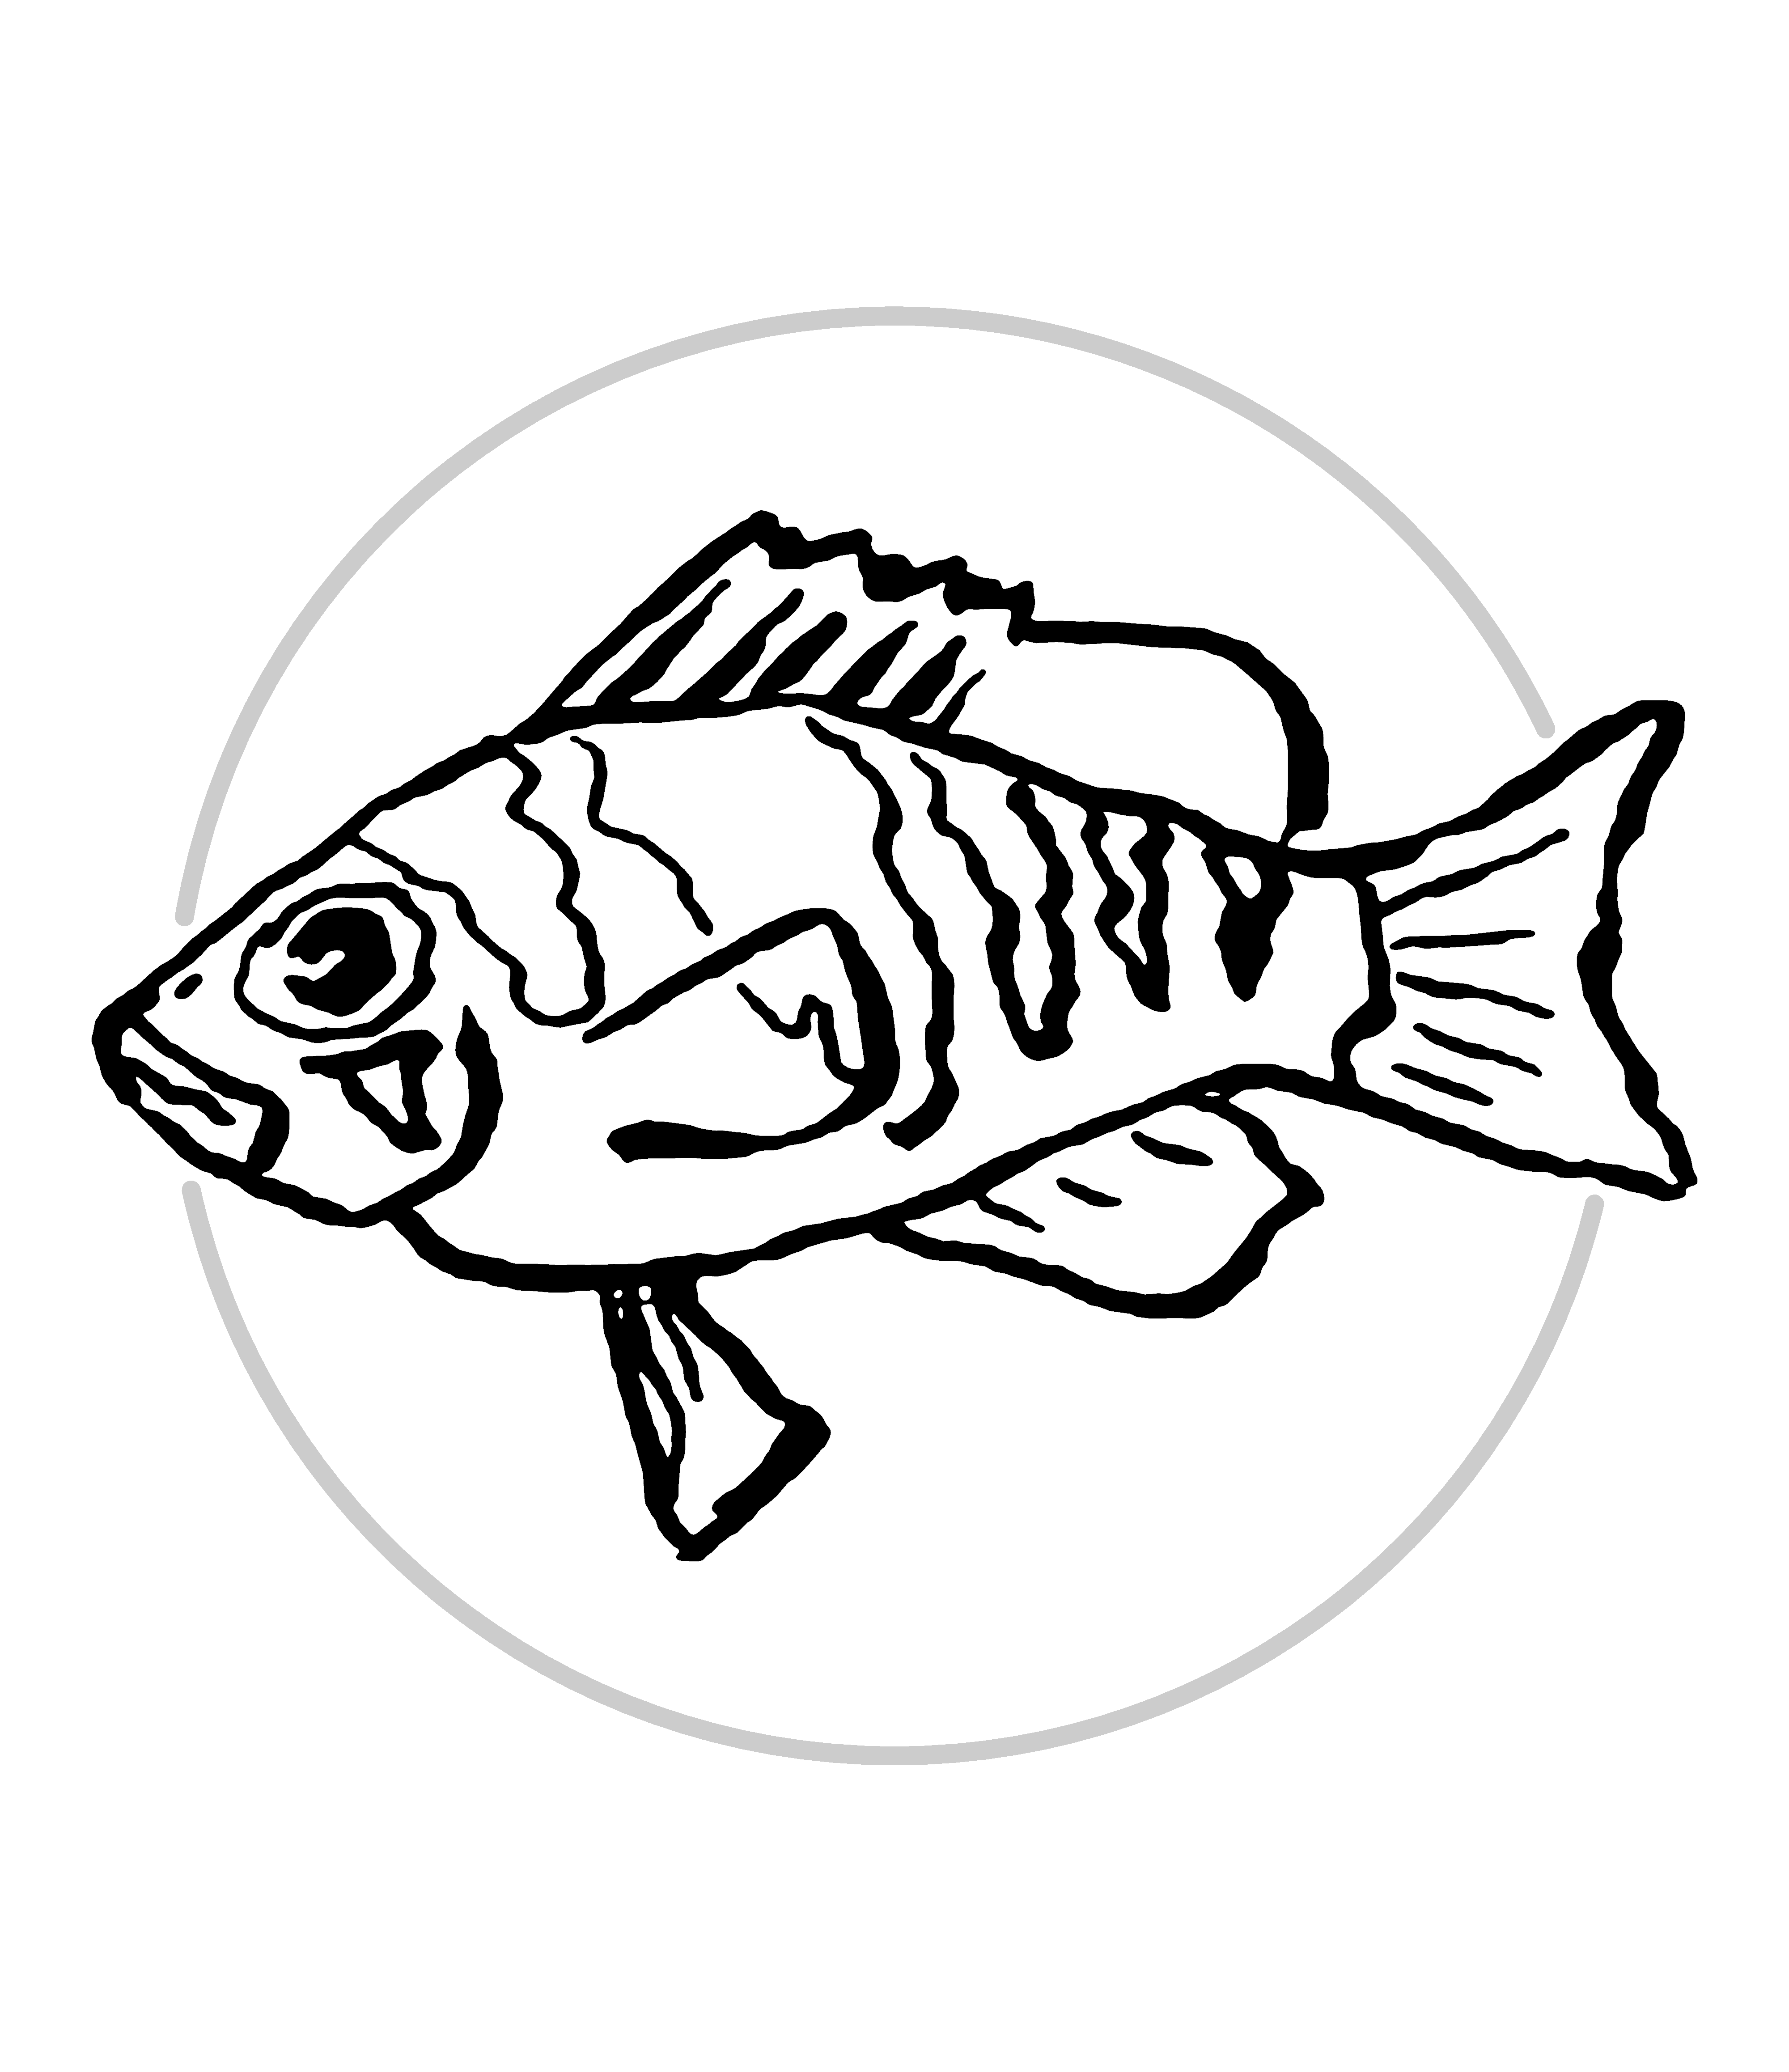
\includegraphics[width = 8em]{images/logo.pdf}
\end{document} 